% Generated by experiments/paper/fig_difficulty.py; do not edit.
\begin{figure*}[t]
\centering
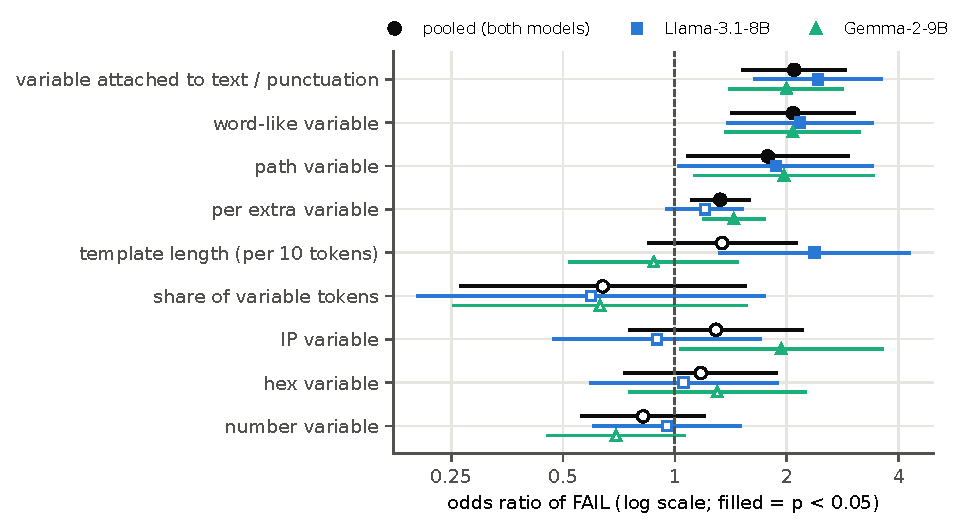
\includegraphics[width=\textwidth]{figures/difficulty.pdf}
\caption{What makes a template hard. Logistic regression of FAIL (main label: fewer than 3 of samples 5--9 match the ground truth exactly) on features of the ground-truth template, over the capped suites of all kept systems (12,500 inputs), with system fixed effects and standard errors clustered by template. Odds ratios with 95\% confidence intervals, pooled over both models (with a model indicator) and per model; filled markers: $p < 0.05$.}
\label{fig:difficulty}
\end{figure*}
